\section{Diagramma delle classi}
L'applicazione SWEDesigner permette di generare un codice Java funzionante a partire da Diagrammi delle classi e diagrammi delle attività.\\
In questa sezione verranno presentati le funzionalità principali offerte dall'applicazione per quanto riguarda la realizzazione di diagrammi delle classi.
	\subsection{Modifica di una classe}
		\begin{figure}[h!]
			\centering
				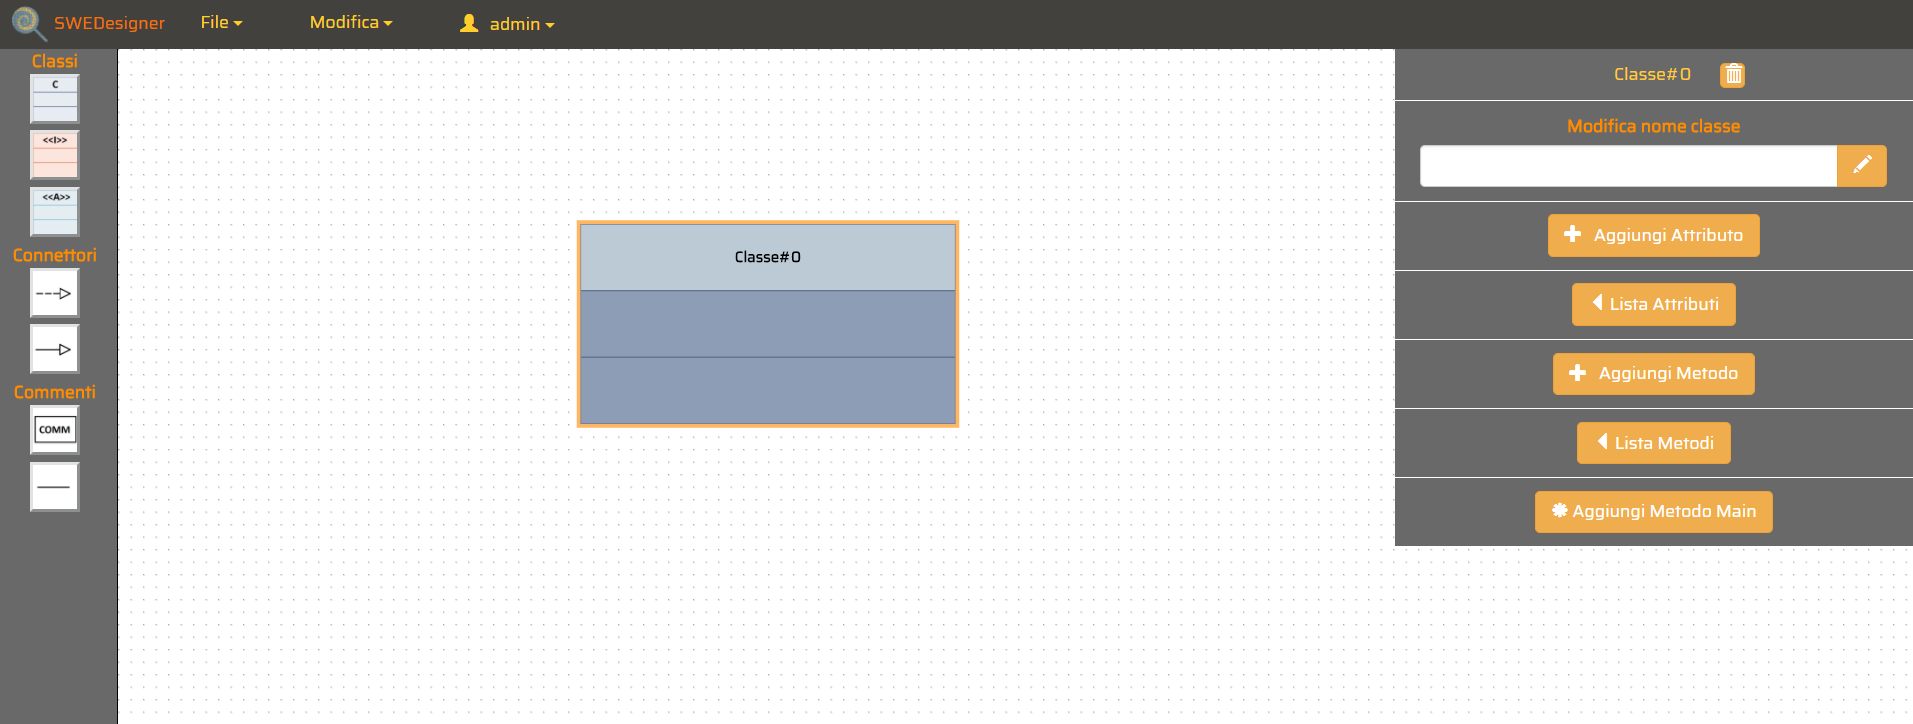
\includegraphics[scale=0.22]{res/img/classe1.png}
			\caption{Modifica di una classe}
		\end{figure}
		Per modificare una classe, una volta cliccato sulla classe desiderata, a destra comparirà un menù di modifica.\\
		Da questo menù è possibile modificare ogni elemento della classe, a partire dal nome che potrà essere modificato inserendo
		un nuovo nome all'interno dell'input \emph{Modifica nome classe} seguito da un click sull'icona della penna situata a fianco dello stesso.\\
		\subsubsection{Aggiunta attributo}
			\begin{figure}[h!]
				\centering
					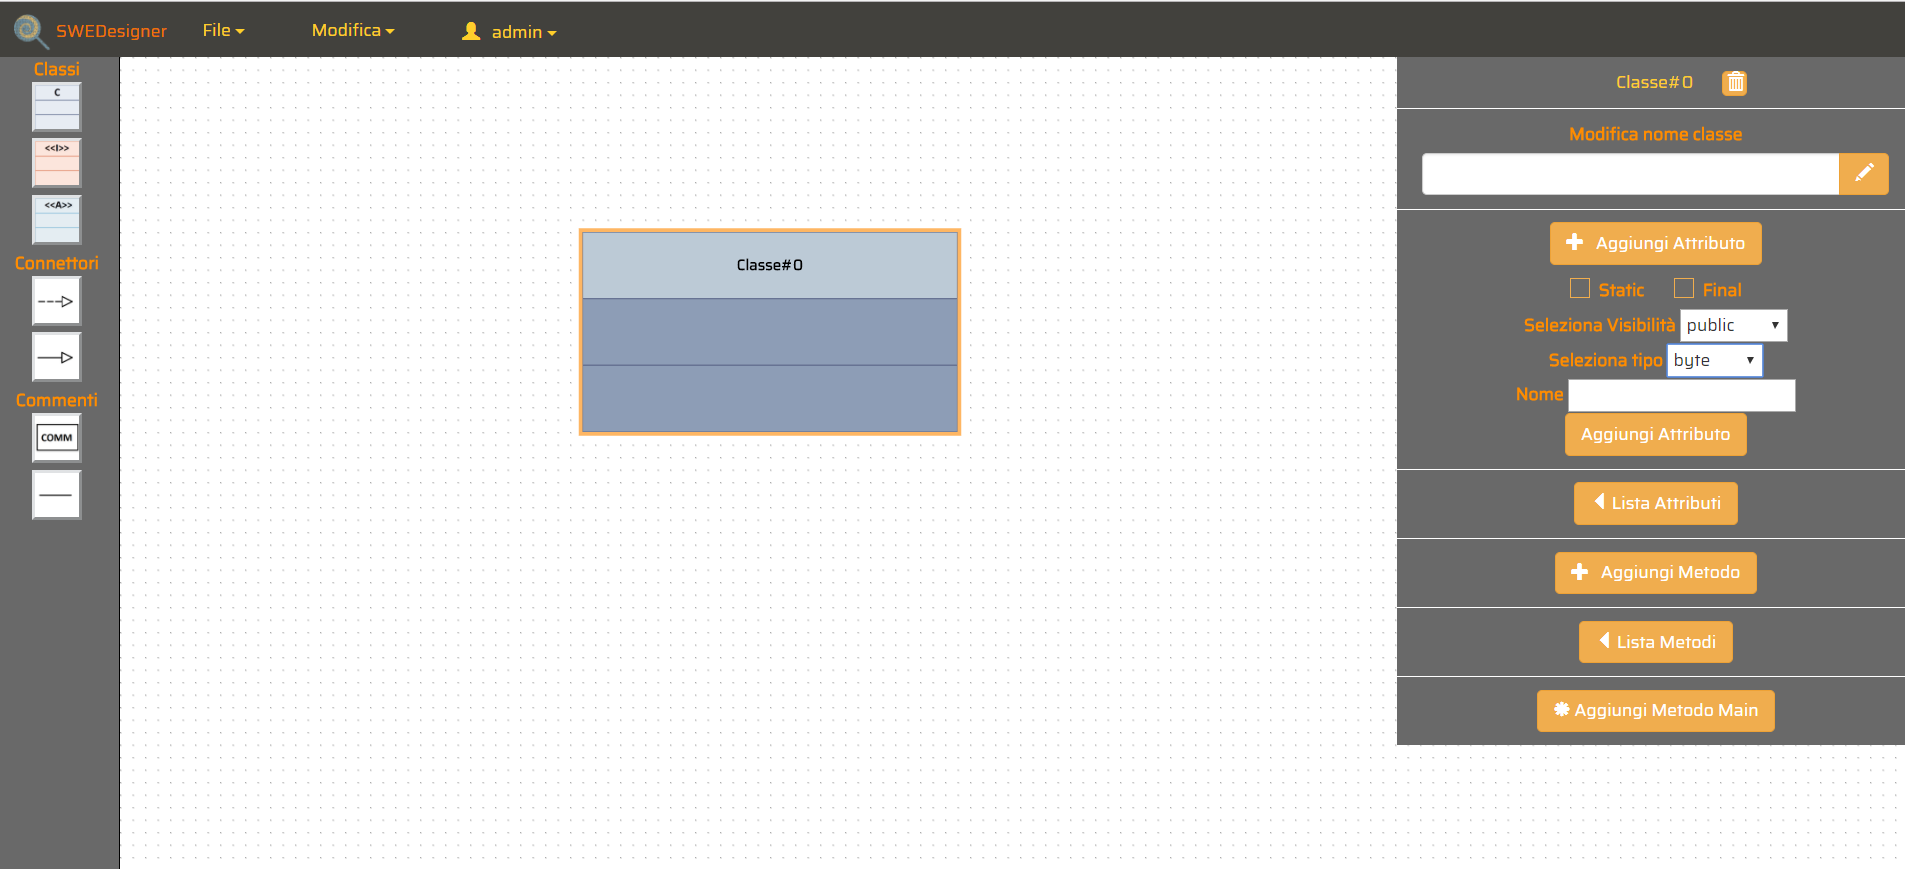
\includegraphics[scale=0.22]{res/img/classe2.png}
				\caption{Modifica di un attributo pt.1}
			\end{figure}
			In questa sezione, accessibile mediante un click su \emph{Aggiungi attributo} è possibile aggiungere un attributo alla classe.\\
			Le opzioni disponibili sono \emph{Static}, mediante la spunta sull'apposito check, \emph{Final}, mediante la spunta sull'apposito check, e normale, senza nessuna spunta.\\
			È possibile selzionare la visibilità dal menù a tendina \emph{Seleziona visibilità} contentente \emph{Private}, \emph{Public} e \emph{Protected}.\\
			È possibile selezionare il tipo primitivo dal menù a tendina \emph{Seleziona Tipo}.\\
			Attraverso l'input \emph{Nome} si aggiunge il nome all'attributo che verrà aggiunto attraverso il click sul bottone \emph{Aggiungi Attributo}.
			Con un click sulla lista attribbuti è possibile aprire una tendina con la possibilità di eliminare l'attributo o di editarlo mediante le stesse funzioni precedentemente descritte.\\
			\begin{figure}[h!]
				\centering
					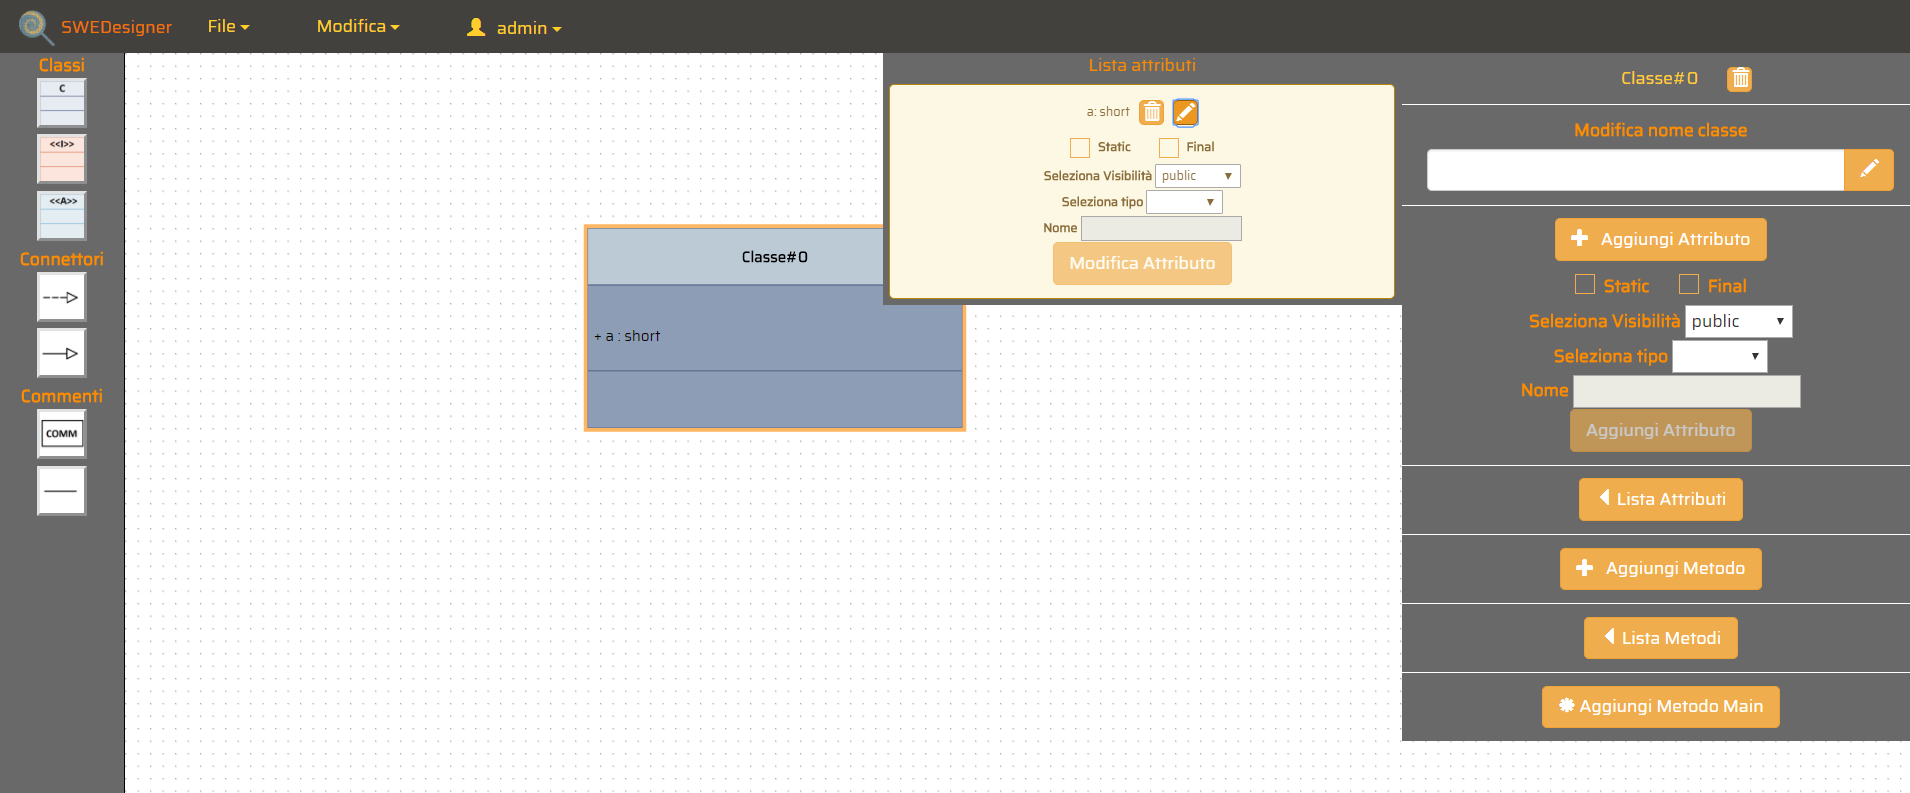
\includegraphics[scale=0.22]{res/img/classe3.png}
				\caption{Modifica di un attributo pt.2}
			\end{figure}
		\subsubsection{Aggiunta metodo}
			\begin{figure}[h!]
				\centering
					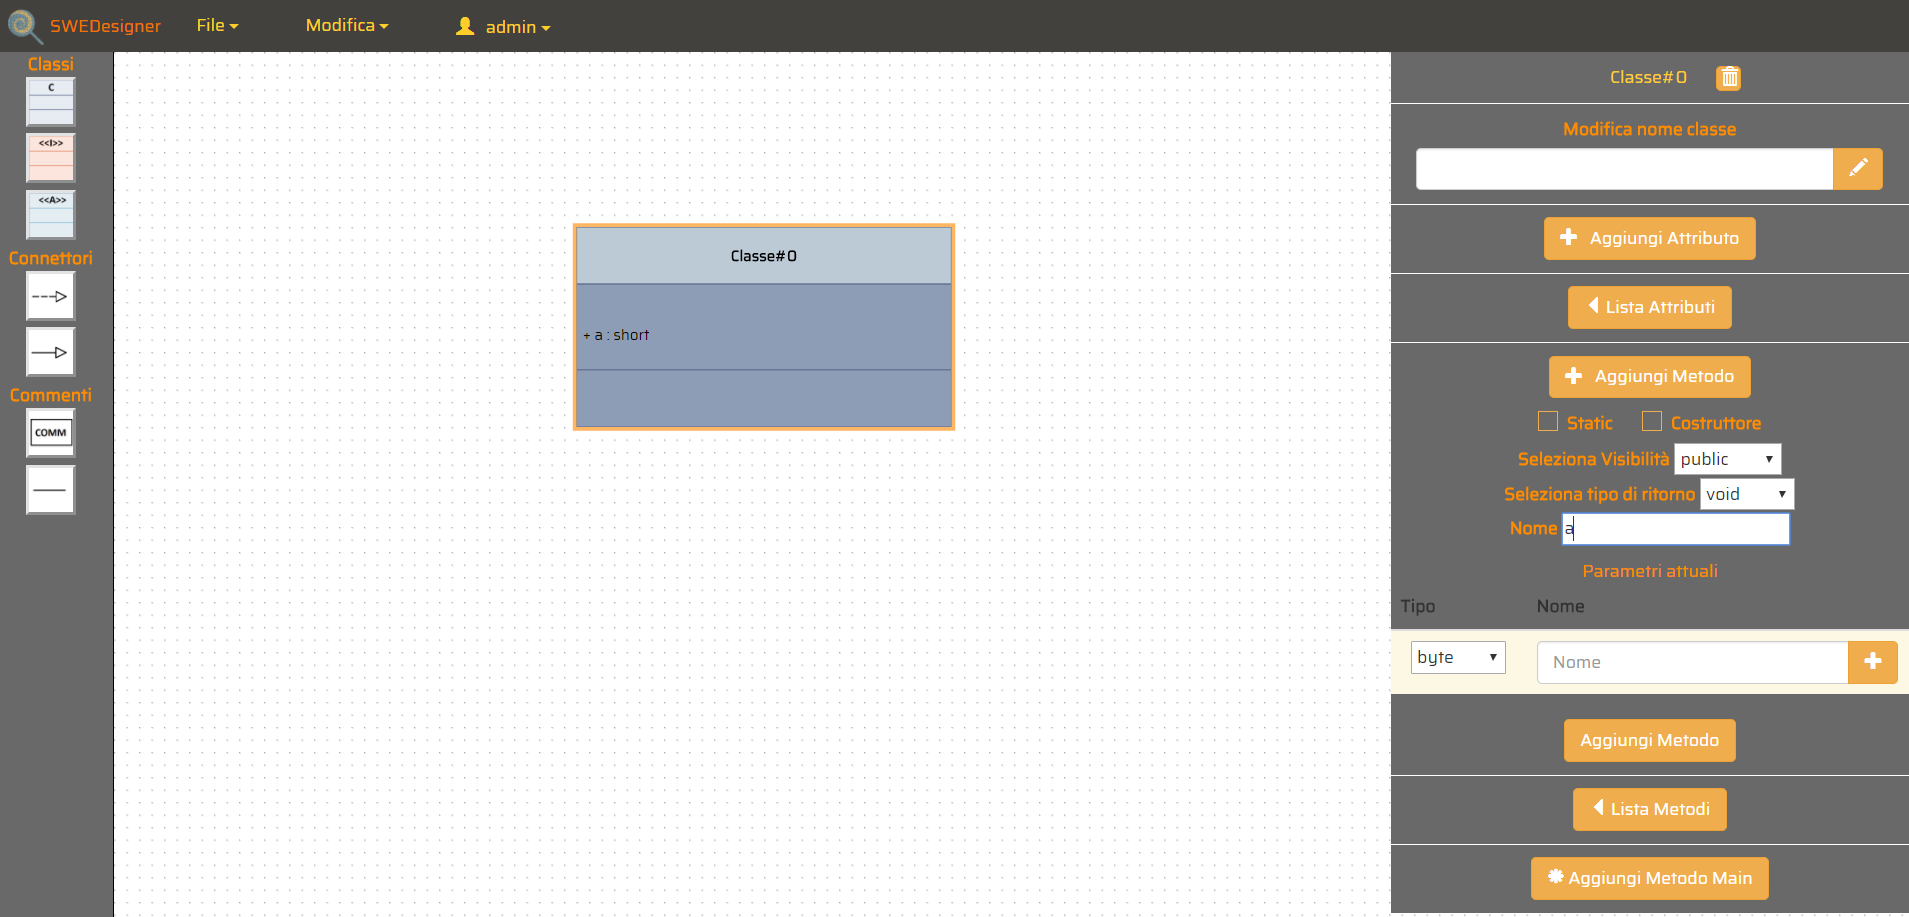
\includegraphics[scale=0.22]{res/img/classe4.png}
				\caption{Modifica di un metodo pt.1}
			\end{figure}
			In questa sezione, accessibile mediante un click su \emph{Aggiungi metodo} è possibile aggiungere un metodo alla classe.\\
			Le opzioni disponibili sono \emph{Static}, mediante la spunta sull'apposito check, \emph{Costruttore}, mediante la spunta sull'apposito check, e normale, senza nessuna spunta.\\
			È possibile selzionare la visibilità dal menù a tendina \emph{Seleziona visibilità} contentente \emph{Private}, \emph{Public} e \emph{Protected}.\\
			È possibile selezionare il tipo di ritorno dal menù a tendina \emph{Seleziona tipo di ritorno}.\\
			Attraverso l'input \emph{Nome} si aggiunge il nome all'attributo e, se necessario, è possibile aggiungere dei parametri attuali al corpo del metodo che verrà aggiunto attraverso il click sul bottone \emph{Aggiungi Metodo}.
			\begin{figure}[h!]
				\centering
					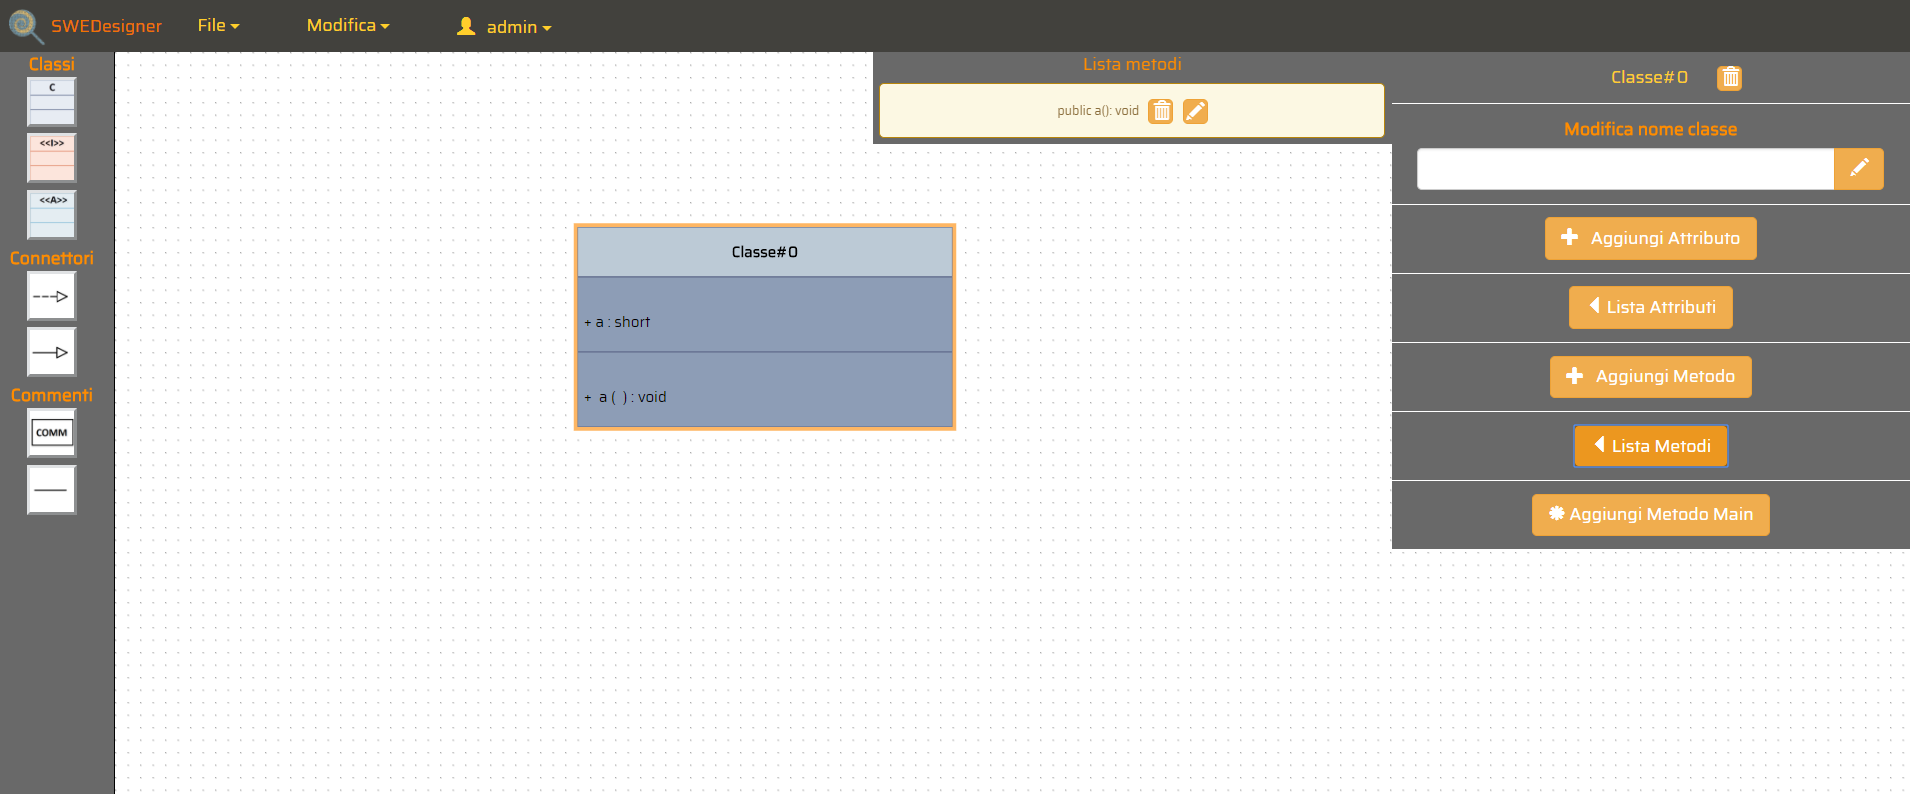
\includegraphics[scale=0.22]{res/img/classe5.png}
				\caption{Modifica di un metodo pt.2}
			\end{figure}
			Con un click sulla lista attribbuti è possibile aprire una tendina con la possibilità di eliminare il metodo o di editarlo mediante le funzionalità che verranno descritte nel prossimo capitolo.
